\documentclass[a4paper,oneside, 11pt]{article}
\usepackage[margin=0.7in]{geometry}
\usepackage[cm-default]{fontspec}
\usepackage{xunicode}
\usepackage{xltxtra}
\usepackage{xgreek}
\usepackage{listings}
\usepackage{hyperref}
\usepackage{parallel,enumitem}
\lstset{basicstyle=\footnotesize\ttfamily,breaklines=true}
\setmainfont[Mapping=tex-text]{CMU Serif}
\usepackage{graphicx}
\usepackage{color}
\usepackage{mathtools, amsmath}
\usepackage{float}
\usepackage{caption}
\usepackage{titling}
\definecolor{codegreen}{rgb}{0,0.6,0}
\definecolor{codegray}{rgb}{0.5,0.5,0.5}
\definecolor{codepurple}{rgb}{0.58,0,0.82}
\definecolor{backcolour}{rgb}{0.95,0.95,0.92}

\lstdefinestyle{mystyle}{
    backgroundcolor=\color{backcolour},   
    commentstyle=\color{codegreen},
    keywordstyle=\color{magenta},
    numberstyle=\tiny\color{codegray},
    stringstyle=\color{codepurple},
    basicstyle=\footnotesize,
    breakatwhitespace=false,         
    breaklines=true,                 
    captionpos=b,                    
    keepspaces=true,                 
    numbers=left,                    
    numbersep=5pt,                  
    showspaces=false,                
    showstringspaces=false,
    showtabs=false,                  
    tabsize=2
}
 
\lstset{style=mystyle}
\makeatletter
\def\maxwidth{%
  \ifdim\Gin@nat@width>\linewidth
    \linewidth
  \else
    \Gin@nat@width
  \fi
}
\makeatother

\makeatletter
\newcommand\xlongleftrightarrow[2][]{%
\ext@arrow 0059{\longleftrightarrowfill@}{#1}{#2}%
}
\def\longleftrightarrowfill@{%
\arrowfill@ ← \relbar → }
\makeatother




\pretitle{%
		\begin{center}
		\LARGE
		
\includegraphics[height=7cm]{pyrforos.png}\\[\bigskipamount]
}
\posttitle{\end{center}}
\title{\textbf{Τεχνητή Νοημοσύνη \\ 1η Προγραμματιστική Εργασία}}
\author{ Ιωάννης Δάρας (\texttt{03115018, el15018@central.ntua.gr, daras.giannhs@gmail.com}) \\
	Μαρία Παρέλλη (\texttt{03115155, el15155@central.ntua.gr})
}
\date{“The key to artificial intelligence has always been the representation.” \\ —Jeff Hawkins}

\newtheorem{theorem}{Theorem}
\begin{document}
\maketitle
\noindent\makebox[\linewidth]{\rule{\paperwidth}{0.4pt}}

\section{Στόχος εργασίας}
Στόχος της συγκεκριμένης εργασίας είναι η χρησιμοποίηση του αλγορίθμου A* ώστε να βρούμε συντομότερες διαδρομές στους δρόμους της Αθήνας. Συγκεκριμένα, έχουμε έναν πελάτη που αναζητά taxi και ένα σύνολο από ταξί σε διαφορετικές τοποθεσίες στην Αθήνα. Ο στόχος είναι να αναθέσουμε στον πελάτη το κοντινότερο σε αυτόν ταξί, ώστε να περιμένει την λιγότερη ώρα.

\section{Αρχιτεκτονική σχεδίασης}
Πριν προχωρήσουμε στις παρακάτω ενότητες, θεωρούμε χρήσιμο να παραθέσουμε την αρχιτεκτονική της λύσης μας για μελλοντική αναφορά. 
Ο πιο απλός τρόπος να εξηγήσουμε την αρχιτεκτονική της λύσης μας είναι παραθέτοντας ένα σχετικό σχήμα.

Συνοπτικά, στο αρχείο Main.java υπάρχει μόνο o driver για τη λύση μας στη συνάρτηση main(). Στο αρχείο Graph.java περιέχεται η καρδιά της υλοποίησης μας. Από τις εσωτερικές κλάσεις, η Graph περιέχει το γράφο που φτιάχνουμε από τα δεδομένα μας και τις μεθόδους createGraph(), createTaxis() για να τον κατασκευάσουμε και run() ως driver της υλοποίησης πάνω στον γράφο. Σημειώνουμε ότι ο γράφος μας περιέχει Nodes τα οποία κληρονομούν από την τάξη Point. Η κλάση Taxi είναι η αντίστοιχη κλάση της Node για τα ταξί. Η κλάση aStar περιέχει την μέθοδο aStarSearch() για να τρέξουμε τον αλγόριθμο aStar και επιστρέφει ένα αντικείμενο τύπου aStarResult που πρακτικά είναι μια δομή που περιέχει τα αποτελέσματα του aStar: το taxi που θα προτιμηθεί, τη διαδρομή που θα ακολουθηθεί και το συνολικό κόστος της διαδρομής. Η κλάση Distance στο αρχείο DIstance.java υλοποιεί τη συνάρτηση υπολογισμού απόστασης. Στο αρχείο KMLExport έχουμε διάφορες χρήσιμες συναρτήσεις για την εξαγωγή των αρχείων KML. \bigbreak

Όλα όσα αναφέρθηκαν συνοπτικά εδώ, αναλύονται με μεγάλη λεπτομέρεια στις επόμενες ενότητες.

\begin{figure}[H]

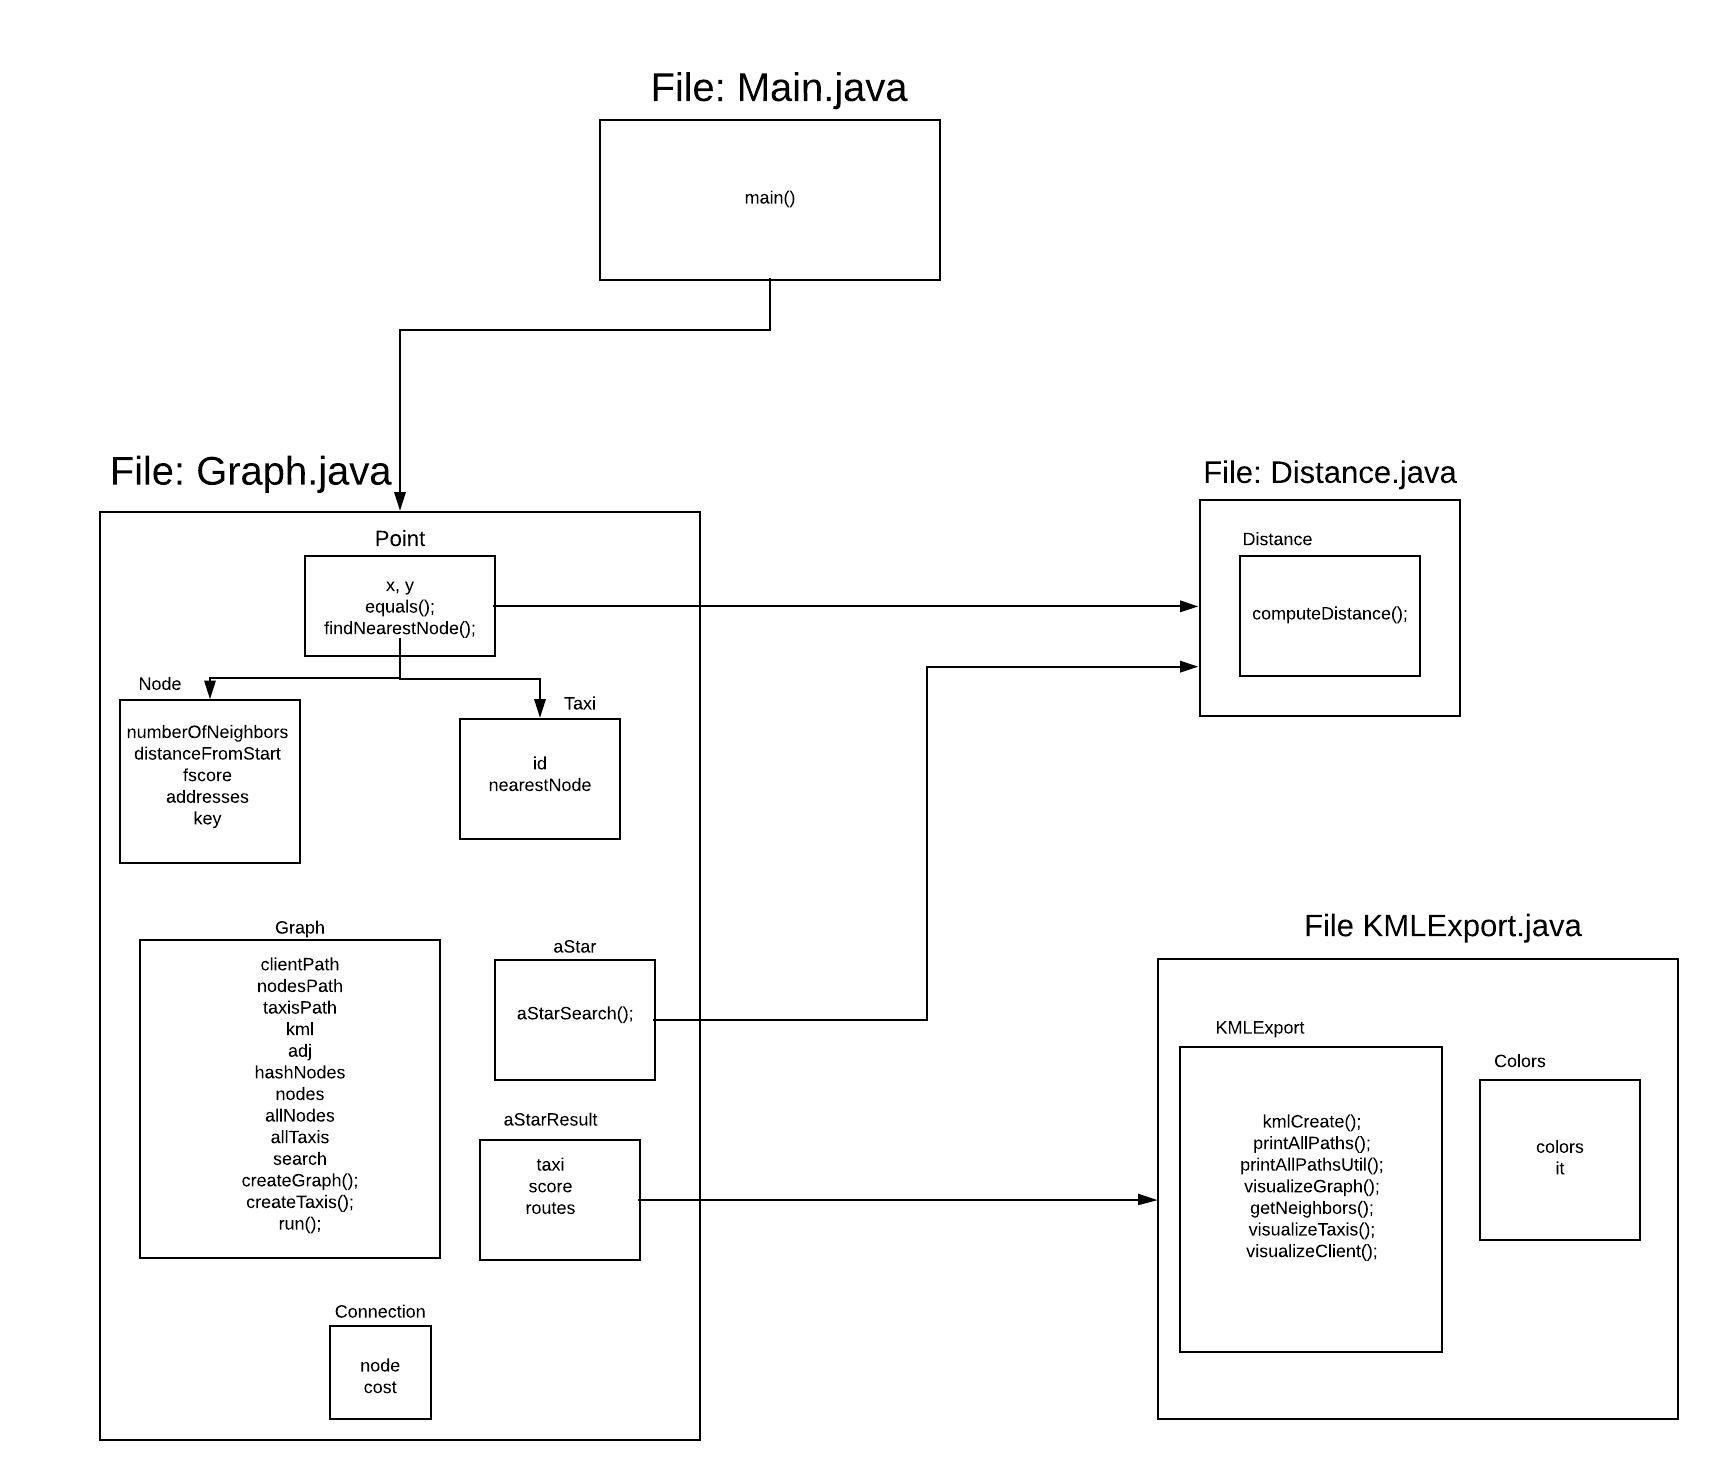
\includegraphics[width=\textwidth]{architecture.jpeg}
\end{figure}




\section{Δεδομένα \& Μοντελοποίηση προβλήματος}
Πρωτού προχωρήσουμε στην ανάλυση των αλγορίθμων θεωρούμε χρήσιμο να αναφέρουμε τον τρόπο που διαχειριζόμαστε τα δεδομένα. \bigbreak 

Το πρόβλημα που εξετάζουμε είναι στατικό, με την έννοια ότι θεωρούμε ότι την ώρα που τρέχουμε τον αλγόριθμο για την εύρεση του κοντινότερου προς τον πελάτη ταξί οι θέσεις του πελάτη και όλων των ταξί μένουν σταθερές και δεν μεταβάλλονται. Αυτές οι θέσεις μπορεί να ενημερώνονται από κάποιο σύστημα GPS με δειγματοληψία περιόδου $\mathcal{T}$, το οποίο όμως στην παρούσα άσκηση θεωρούμε ότι δεν μας ενδιαφέρει. \bigbreak

Οι στατικές θέσεις του πελάτη και των ταξί δίνονται με τη μορφή csv αρχείων. Συγκεκριμένα, έχουμε το αρχείο client.csv το οποίο περιέχει τις γεωγραφικές συντεταγμένες του client, το αρχείο taxis.csv το οποίο περιέχει τις γεωγραφικές συντεταγμένες των taxi και το id της διεύθυνσης στην οποία βρίσκονται και τέλος το αρχείο nodes.csv που πρακτικά αποτελεί μια δειγματοληψία στο χώρο των σημείων των δρόμων της Αθήνας και περιέχει τις γεωγραφικές συντεταγμένες των διαφόρων σημείων, την διεύθυνση στην οποία αυτά βρίσκονται, και πιθανώς, το όνομα της συγκεκριμένης διεύθυνσης. Στην παρούσα άσκηση μας αρκούν μόνο τα αριθμητικά δεδομένα και συνεπώς δεν χρησιμοποιούμε καθόλου την πληροφορία του ονόματος της διεύθυνσης.  \bigbreak 

 

\subsection{Προεπεξεργασία δοθέντων δεδομένων}
Τα δεδομένα που μας δίνονται περιέχουν στην πρώτη γραμμή τους ένα header που πληροφορεί για το είδος της πληροφορίας κάθε στήλης του csv αρχείου. Αυτά τα headers δεν μας ενδιαφέρουν καθώς γνωρίζουμε το είδος της αντίστοιχης πληροφορίας και συνεπώς τα αφαιρούμε για διευκόλυνση. \bigbreak 

Στο σημείο αυτό, προχωράμε σε μια στατιστική ανάλυση των δεδομένων που μας δίνονται.
\subsection{Στατιστική ανάλυση δεδομένων}
Αρχικά, εκτελώντας τις παρακάτω bash εντολές μπορούμε να μετρήσουμε το σύνολο των γραμμών των αρχείων nodes.csv και taxis.csv

\begin{lstlisting}[language=Bash]
wc -l nodes.csv
wc -l taxis.csv
\end{lstlisting}

Παρατηρούμε ότι έχουμε $\approx 15000$ nodes και 11 ταξί. Τα nodes αυτά \underline{δεν} είναι μοναδικά. Ορισμένα σημεία ανήκουν σε διασταυρώσεις και συνεπώς εμφανίζονται παραπάνω από μια φορές. \bigbreak 

Η μοντελοποίηση που επιχειρούμε είναι να φτιάξουμε έναν γράφο που θα περιέχει ως κόμβους μόνο τα διακριτά σημεία (διακριτά ζευγάρια συντεταγμένων (X,Y)) και για το κάθε σημείο θα υπάρχει ένα adjacency list με άλλα σημεία που γειτονεύει. \bigbreak 

Το πραγματικό ερώτημα είναι τι ορίζουμε ως γειτνίαση στη συγκεκριμένη περίπτωση. Η απάντηση που εμείς προτείνουμε είναι ότι κάθε σημείο διασταύρωσης θα γειτνιάζει με όλα τα σημεία που βρίσκονται και αυτά στην ίδια διασταύρωση και ότι κάθε σημείο ενός δρόμου θα γειτνιάζει με το αμέσως επόμενο σημείο (όπως τα διαβάζουμε σειριακά από το αρχείο) που είναι στον ίδιο δρόμο. \bigbreak 

Κανονικά, μια τέτοια αναπαράσταση θα προϋπόθετε χρονική πολυπλοκότητα $O(n^2)$, όπου n ο αριθμός των σειρών στο αρχείο nodes.csv. Όμως, τα δεδομένα μας δίνονται με μια συγκεκριμένη σειρά. Συγκεκριμένα, αν το σημείο με id x βρίσκεται στην ίδια διασταύρωση με τα σημεία με id y, z τότε το αρχείο θα έχει την ακόλουθη σειρά γραμμών:
$$\textrm{<longtitude\_x> <latitude\_x> <addr>}$$
$$\textrm{<longtitude\_y> <latitude\_y> <addr>}$$
$$\textrm{<longtitude\_x> <latitude\_x> <addr>}$$
$$\textrm{<longtitude\_z> <latitude\_z> <addr>}$$
Αυτό σημαίνει ότι για ένα συγκεκριμένο σημείο x δεν χρειάζεται να ψάξουμε όλο το γράφο για να βρούμε τους γείτονες του αλλά μόνο το επόμενο σημείο στο αρχείο nodes.csv. \bigbreak

Έτσι, η συνολική πολυπλοκότητα κατασκευής του γράφου γίνεται:
$$O(n)$$

\subsection{Μοντελοποίηση σε επίπεδο κώδικα}

Στην ενότητα αυτή, περιγράφουμε τις δομές που χρησιμοποιήθηκαν προκειμένου να μοντελοποιηθούν τα δεδομένα με τον τρόπο που περιγράψαμε. Αρχικά, στη μεταβλητή allNodes βάζουμε όλα τα nodes που διαβάζουμε από το csv αρχείο με έναν csvReader σε java από το αρχείο nodes.csv . Αντίστοιχα, στη μεταβλητή allTaxis βάζουμε όλα τα taxis που διαβάζουμε από το αρχείο taxis.csv . Για κάθε node και κάθε taxi θέλουμε ένα id για να μπορούμε να το προσδιορίσουμε μοναδικά. Για τα taxi το id αυτό μπορεί να είναι το id της διεύθυνσης στην οποία βρίσκονται αρχικά καθώς δεν βρίσκονται δύο ταξί στην ίδια αρχική διεύθυνση (αν θεωρήσουμε ότι αυτό το σενάριο μπορεί να συμβεί τότε πάλι τους δίνουμε το ίδιο id καθώς δεν μας ενδιαφέρει η διάκριση μεταξύ των ταξί). Όπως είπαμε, η μεταβλητή allNodes περιέχει όλα τα nodes που υπάρχουν στο csv αρχείο. Αυτά τα nodes όμως πολλές φορές αντιστοιχούν στο ίδιο σημείο. Προκειμένου να μην έχουμε στο γράφο μας duplicate nodes, φτιάχνουμε τη μεταβλητή nodes η οποία περιέχει μόνο τα διακριτά Nodes του χάρτη. \bigbreak 


Επειδή κάθε Node και κάθε Taxi είναι πρώτα ένα Point, φτιάχνουμε και την κλάση Point ως γονέα των Node, Taxi. Η κλάση αυτή υλοποιεί και τη συνάρτηση findNearestNode(). Η συνάρτηση αυτή είναι ιδιαίτερα χρήσιμη για τον A* που θα αναλύσουμε αργότερα καθώς μπορεί κάποιο taxi ή ο client να μην είναι σημεία του γράφου. Αυτή η συνάρτηση παίρνει ως είσοδο ένα τέτοιο σημείο και μας επιστρέφει το κοντινότερο σημείο του στο γράφο. \bigbreak 

Αφού μιλήσαμε για τις μεταβλητές allNodes, allTaxis, hashNodes, nodes και την κλάση Point μένει μόνο να εξηγήσουμε τη μεταβλητή 
adj. Η μεταβλητή αυτή πρακτικά είναι το adjacency list του γράφου μας. Με είσοδο έναν αριθμό τύπου Long, που αντιστοιχεί στο node id, μας επιστρέφει μια λίστα από τους γείτονες του συγκεκριμένου Node όπου κάθε γείτονας αντιστοιχεί σε ένα αντικείμενο της κλάσης Connectio. H κλάση Connection έχει ως πεδία τον γείτονα και το κόστος της γειτνίασης. Το κόστος αυτό υπολογίζεται από την στατική κλάση Distance που υπολογίζει κόστος μεταξύ σημείων. Η μεταβλητή adj φτιάχνεται όπως αναφέραμε παραπάνω, δηλαδή ενώνοντας τα nodes που αντιστοιχούν σε διαδοχικές γραμμές του αρχείο nodes.csv . Σημειώνουμε πως κάνουμε τον γράφο κατευθυνόμενο για μελλοντική πιθανή επέκταση, αλλά στην πραγματικότητα όλες οι συνδέσεις έχουν και τις δύο φορές, δηλαδή στους δρόμους δεν ορίζουμε επιτρεπόμενη κατεύθυνση στην παρούσα φάση καθώς μια τέτοια πληροφορία δεν είναι διαθέσιμη.

\section{Αλγόριθμος A*}
Αρχικά, αναφέρουμε τον κλασσικό αλγόριθμο A* και στη συνέχεια σημειώνουμε τα σημεία στα οποία η δική μας υλοποίηση διαφέρει καθώς και τους λόγους των σχεδιαστικών επιλογών που κάνουμε. \bigbreak 

Ο κλασσικός αλγόριθμος A*, όπως και οι περισσότεροι αλγόριθμοι αναζήτησης καλύτερου μονοπατιού, χρησιμοποιεί δύο δομές: το ανοικτό μέτωπο, για τους κόμβους του γράφου που έχει ανακαλύψει αλλά δεν έχει διευρύνει και το κλειστό σύνολο για τους κόμβους του γράφου που έχει ανακαλύψει και διευρύνει πλήρως. Στον A*, το ανοικτό μέτωπο είναι διατεταγμένο ως προς την τιμή της συνάρτησης f για τον κάθε κόμβο. Η συνάρτηση αυτή ορίζεται πάνω σε ένα γράφο G(V, E)
$$
f(n) = g(n) + h(n), \quad n\in V
$$
όπου g(n,s) είναι το κόστος που έχουμε πληρώσει ως τώρα για να φτάσουμε στον κόμβο n και h(n) είναι η τιμή μιας ευριστικής συνάρτησης-εκτιμήτριας για το πόσο μακριά είναι ο κόμβος n από τον στόχο. \bigbreak

Ο αλγόριθμος A* κάθε φορά διαλέγει το σημείο με τη μικρότερη τιμή της συνάρτησης f και και ανανεώνει τις τιμές των γειτόνων του. Ο αλγόριθμος τερματίζει όταν βρεθεί ο κόμβος προορισμού ή όταν αδειάσει το ανοικτό μέτωπο.

\subsection{Διαφορές από τον κλασσικό αλγόριθμο}

Ο αλγόριθμος που υλοποιούμε έχει κάποιες διαφορές από τον κλασσικό αλγόριθμο A*, οι οποίες έχουν τις ρίζες τους στη θέληση μας για:
\begin{itemize}
\item Πολλαπλούς στόχους. \par 
Ο κλασσικός αλγόριθμος A* τρέχει από έναν κόμβο (source) προς έναν κόμβο (destination). Εμείς όμως θέλουμε να τρέξουμε A* από έναν κόμβο (source) που αντιστοιχεί στον πελάτη, προς πολλούς κόμβους (destination\textbf s), που αντιστοιχούν στα taxi. 
\item Εναλλακτικές διαδρομές. \par 
Στον κλασσικό αλγόριθμο A* βρίσκουμε μια διαδρομή από τον source node προς τον destination node. Εδώ θέλουμε να βρούμε διαφορετικές, πιθανώς ισοδύναμες διαδρομές για να προτείνουμε.
\end{itemize}


\subsection{Βελτιστότητα A*}
Σε αυτή την ενότητα αναφέρουμε μια θεμελίωδη ιδιότητα του A* που θα μας φανεί ιδιαίτερα χρήσιμη για τις ιδέες υλοποίησης που εκφράζουμε παρακάτω. \bigbreak 


\begin{theorem}
Αν η εκτιμήτρια συνάρτηση δεν υπερεκτιμά ποτέ το κόστος μεταξύ του κόμβου και του τελικού στόχου τότε ο A* εγγυάται βέλτιστη λύση.
\end{theorem}




\subsection{Ιδέες υλοποίησης}
Στην ενότητα αυτή παρουσιάζουμε τις βασικές ιδέες υλοποιήσης που χρησιμοποιούμε προκειμένου να προσθέσουμε στη δική μας παραλλαγή του A* τις επιθυμητές ιδιότητες που αναφέραμε. 

\begin{itemize}
\item Πολλαπλοί στόχοι. \bigbreak 
Η βασική ιδέα συνοψίζεται στη μαθηματική σχέση:
$$
h(n) = min\{ \forall d_i \in D: h(n | d_i) \}
$$
Η μαθηματική αυτή σχέση μας λέει ότι για την τιμή της ευριστικής για ένα node παίρνουμε το minimum από τις ευριστικές που θα προέκυπταν αν είχαμε έναν οποιονδήποτε στόχο (και όχι πολλούς). \bigbreak 

Πρακτικά, κάθε φορά που εξετάζουμε λοιπόν έναν κόμβο, υπολογίζουμε το heuristic του ως προς όλα τα taxi και παίρνουμε το μικρότερο. \bigbreak 

Αυτή η ευριστική είναι κατάλληλη για πολλαπλούς στόχους καθώς αν η ευριστική για ένα στόχο δεν κάνει ποτέ υπερεκτίμηση τότε και η ευριστική για πολλαπλούς στόχους δεν θα κάνει ποτέ υπερεκτίμηση λόγω του τελεστή min. \bigbreak 

\item Εναλλακτικές διαδρομές \bigbreak 

Προδιαγραφή της υλοποίησης είναι να βρίσκουμε και εναλλακτικές ισοδύναμες διαδρομές, εφόσον αυτές υπάρχουν. Επειδή χρησιμοποιούμε floats, δεν θα βρούμε ποτέ πραγματικά ισοδύναμες διαδρομές. Έτσι, ορίζουμε μια μικρή ποσότητα ως $tolerance$ για το πότε δύο διαδρομές θεωρούνται ισάξιες. Κάνοντας διάφορα πειράματα, είδαμε ότι η καλύτερη τιμή δια την μεταβλητή tolerance κυμαίνεται στο διάστημα:
$[2,10]$m. \bigbreak 

Για τον υπολογισμό των εναλλακτικών διαδρομών, κάθε φορά που επεκτείνουμε έναν κόμβο από το μέτωπο αναζήτησης και εξετάζουμε ένα γείτονα του κάνουμε τους ελέγχους που περιγράφονται στο ακόλουθο διάγραμμα ροής. Συμβολίζουμε με $f'$ την καινούργια υπολογιζόμενη τιμή για τον κόμβο n προερχόμενοι από τον s, και f την παλιά.

\begin{figure}[H]

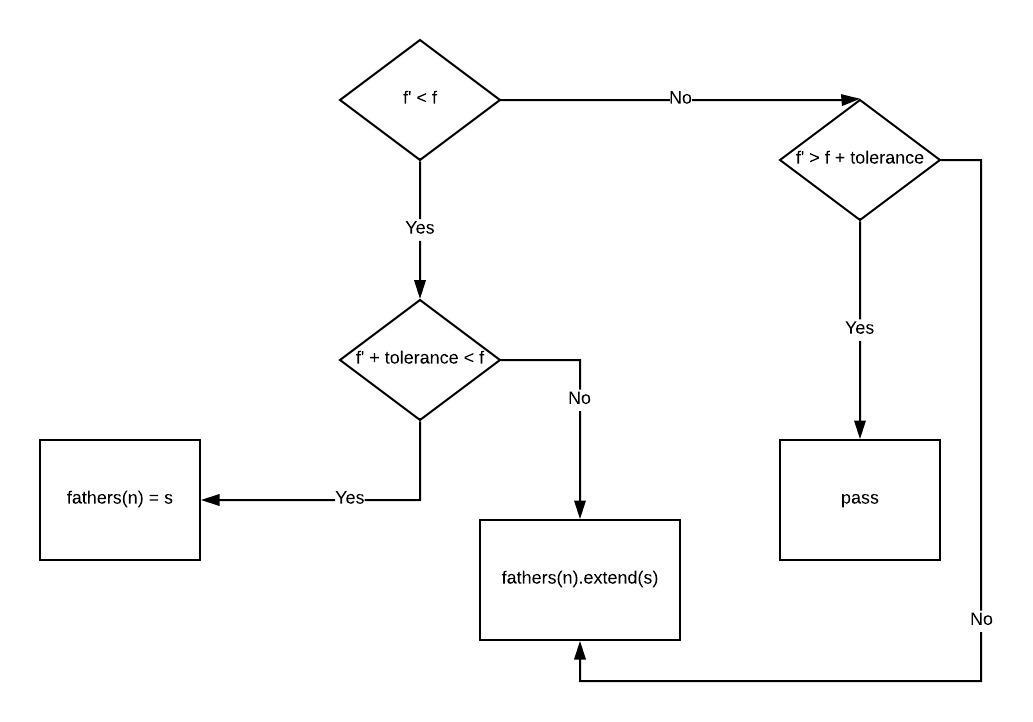
\includegraphics[width=\textwidth]{diagramma_rois.jpeg}
\end{figure}

\end{itemize}


Ακολουθώντας αυτή την τακτική, επιτρέπουμε να δημιουργηθούν παρακλάδια στην βέλτιστη διαδρομή που καθένα από αυτά δημιουργεί μια νέα διαδρομή που θεωρείται ισοδύναμη.


\subsubsection{Υπολογισμός απόστασης και ευριστική συνάρτηση}
Οι τελευταίες ιδέες υλοποίησης που αξίζει να αναφέρουμε είναι το είδος του υπολογισμού απόστασης και το είδος της ευριστικής συνάρτησης που χρησιμοποιούμε. \bigbreak 

Για τον υπολογισμό της απόστασης θεωρούμε ότι η Γη είναι σφαίρα και χρησιμοποιούμε την Haversine απόσταση:
$$
D(x, y) =  2 r arcsin\left( \sqrt{  sin^2(\frac{\phi_2 - \phi_1}{2}) + cos(\phi_2)\cdot cos(\phi_1)sin^2(\frac{\lambda_2 - \lambda_1}{2} )        }\right)
$$
όπου τα φ αναπαριστούν τα γεωμετρικά πλάτη και τα λ τα γεωμετρικά μήκη. \bigbreak 

Ως ευριστική συνάρτηση χρησιμοποιούμε την: 
$$
H(x, y) = k \cdot D(x,y), \quad x \in (0, 1)
$$

Αυτό σημαίνει ότι χρησιμοποιούμε πάλι την Haversine αλλά πολλαπλασιασμένη με έναν παράγοντα k ώστε να είναι μικρότερη από την πραγματική απόσταση και να ικανοποιείται η αρχή της βελτιστότητας που αναφέραμε για τον αλγόριθμο A*.


\subsection{Υλοποίηση σε επίπεδο κώδικα}
Η απόσταση Haversine υλοποιείται στο αρχείο Distance.java στην κλάση Distance μεταξύ σημείων Points. Instances των σημείων μπορεί να είναι όλες οι κλασεις παιδιά, δηλαδή τα Nodes και τα Taxis. Η υλοποίηση του aStar γίνεται στην κλάση aStar στη μέθοδο aStarSearch. Ο αρχικός κόμβος είναι ο πλησιέστερος κόμβος στον client που υπολογίζεται μέσω της συνάρτησης findNearestNode της κλάσης Point. Οι τελικοί κόμβοι είναι οι πλησιέστεροι κόμβοι του γράφου στα αντικείμενα της μεταβλητής allTaxis. Τα κλειδιά των τελικών κόμβων αποθηκεύονται στο endKeys ενώ η αντιστοίχηση μεταξύ των κλειδιών των τελικών κόμβων και των κλειδιών των taxis γίνεται στο HashMap taxiKeysMap. Το κλειστό σύνολο υλοποιείται ως HashSet από Nodes στην μεταβλητή visited. Το ανοικτό μέτωπο υλοποιείται ως Treeset από Nodes. Ο λόγος που χρησιμοποιούμε Set είναι για να αποφύγουμε τα duplicates. Ο λόγος που χρησιμοποιούμε TreeSet είναι ότι θέλουμε να έχουμε διατεταγμένο ανοικτό μέτωπο. Τη συνάρτηση διάταξης την ορίζουμε εμείς μέσω ενός Comparator χρησιμοποιώντας το fscore των Nodes. Για τα updates χρησιμοποιούμε τη λογική των tolerance όπως την εκφράσαμε παραπάνω. Μια δομή που αξίζει να αναφέρουμε είναι η δομή parentsMap που παίρνει ένα id και το αντιστοιχίζει (HashMap) σε ένα HashSet από father nodes όπως ακριβώς περιγράψαμε παραπάνω.  \bigbreak 

Το αποτέλεσμα της aStarSearch είναι μια μεταβλητή της κλάσης aStarResult και περιέχει τη δομή parentsMap, το taxiId που επιλέχθηκε και το συνολικό κόστος της διαδρομής. 


\section{KMLExports}
Αφού πάρουμε το αποτέλεσμα του A* πρέπει να το κάνουμε export κατάλληλα σε ένα KML αρχείο ώστε να το προβάλλουμε στο OpenMaps της Google. Οι συναρτήσεις που αφορούν την οπτικοποιήση των αποτελεσμάτων είναι στο αρχείο KMLExport.java. Στο αρχείο αυτό ορίζονται δύο κλάσεις. Η πρώτη από αυτές, η κλάση Colors, έχει πρακτικά έναν iterator πάνω σε strings για colors που χρησιμοποιούμε προκειμένου να χρωματίσουμε με διαφορετικό χρώμα τις ισοδύναμες διαδρομές. Η δεύτερη κλάση, η KMLExport, περιέχει όλες τις συναρτήσεις οπτικοποίησης των αποτελεσμάτων. Συγκεκριμένα:

\begin{itemize}
\item visualizeGraph(): μια συνάρτηση απεικόνισης σε kml αρχείο όλων των κόμβων του δειγματοληπτημένου γράφου της εκφώνησης. Το kml αρχείο που προκύπτει είναι 12 MB και συνεπώς δεν μπορούμε να το οπτικοποιήσουμε δωρεάν με την υπηρεσία my maps, παρόλα αυτά το παραθέτουμε. 
\item visualizeTaxis(): η συνάρτηση αυτή είναι για τη δημιουργία ενός kml αρχείου απεικόνισης όλων των taxi. Για τα taxi, χρησιμοποιούμε ένα custom design σε μορφή πινέζας, ώστε να τα ξεχωρίζουμε από τον Client στο χάρτη. Η εικόνα για τα ταξί που μας δίνονται στην εκφώνηση είναι η ακόλουθη:

\begin{figure}[H]
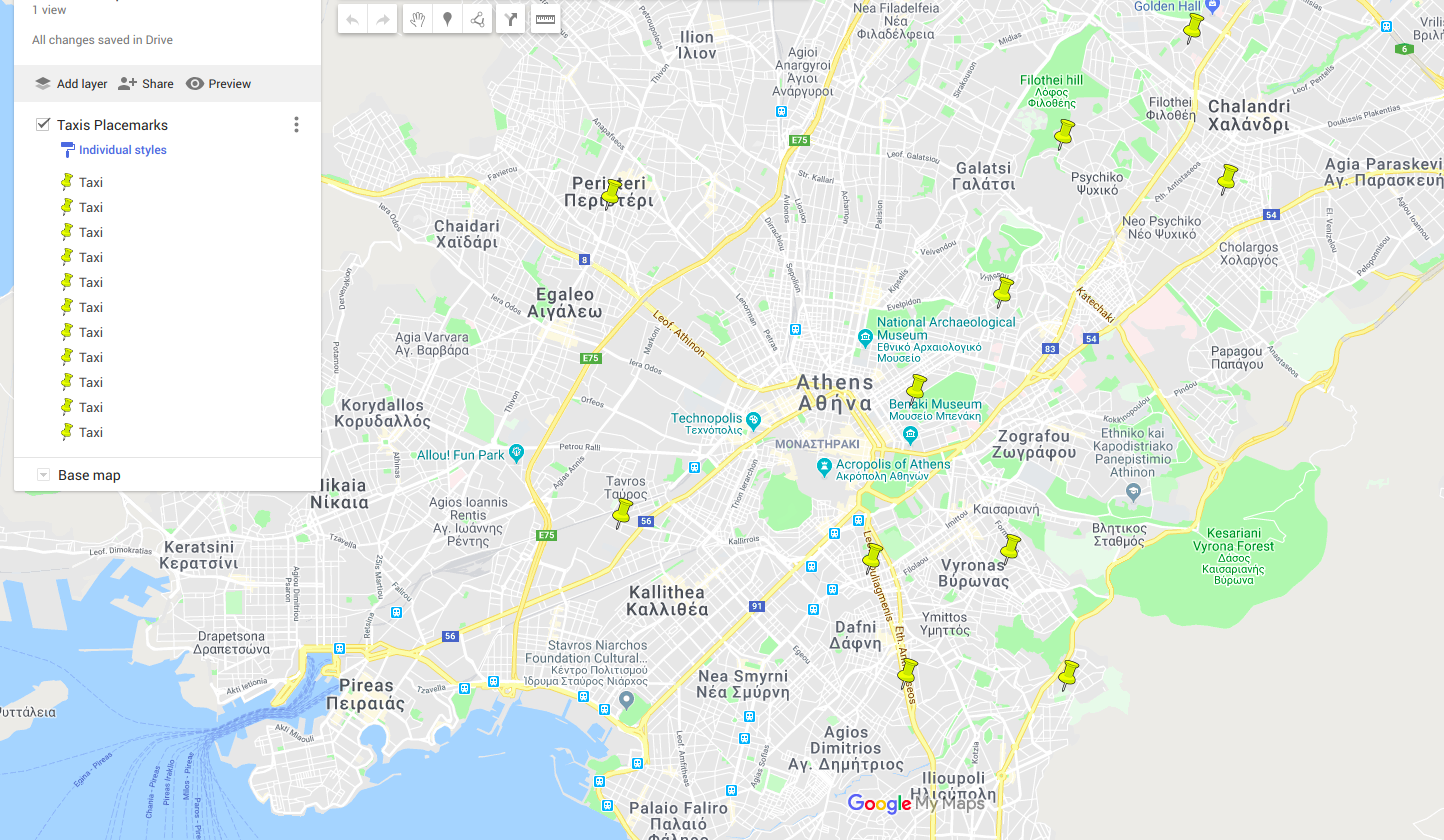
\includegraphics[width=\textwidth]{taxis.png}
\end{figure}


\item visualizeClient(): η συνάρτηση αυτή είναι για τη δημιουργία ενός kml αρχείου για την οπτικοποίηση του Client. Η εικόνα για τον client που μας δίνεται στα δεδομένα της άσκησης φαίνεται παρακάτω:


\begin{figure}[H]
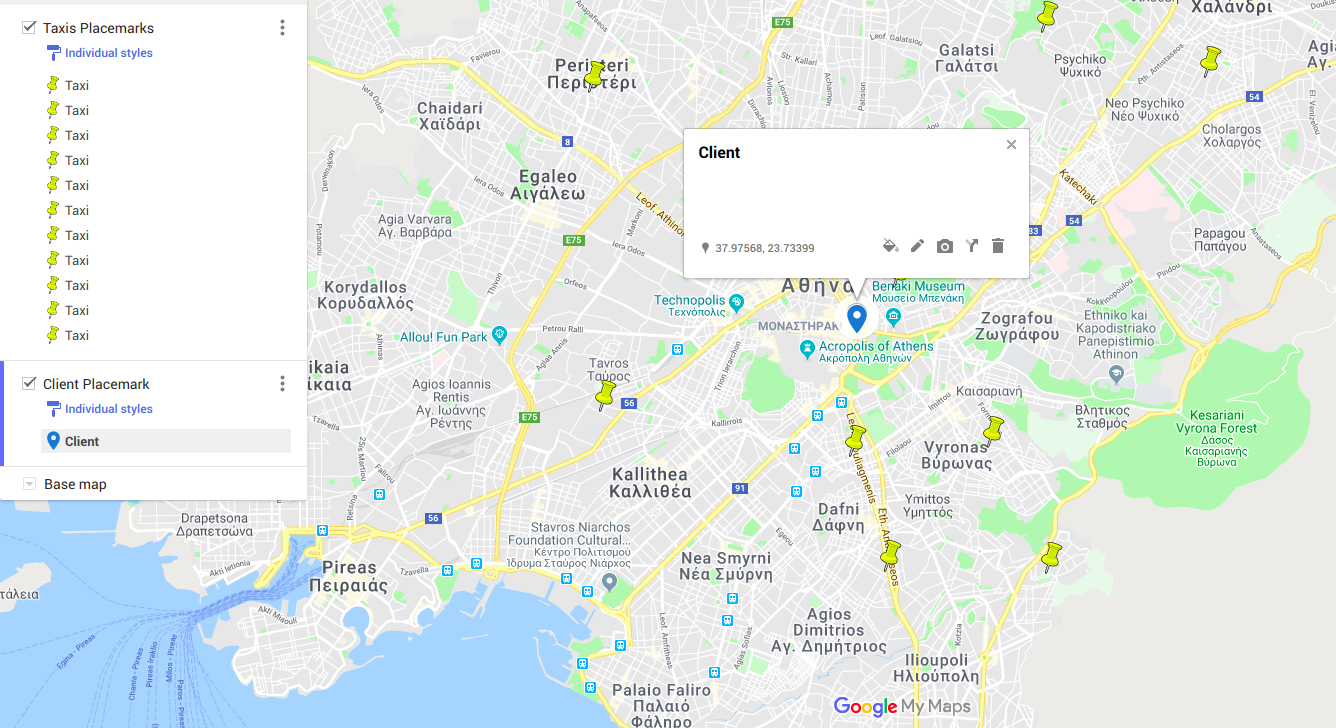
\includegraphics[width=\textwidth]{client.png}
\end{figure}

\item kmlCreate(): η συνάρτηση απεικόνισης των εναλλακτικών διαδρομών από έναν αρχικό κόμβο σε έναν τελικό. Η συνάρτηση αυτή χρησιμοποιεί τη μεταβλητή routes που είναι το parentsMap που κατασκευάσαμε κατά τον A*. Συγκεκριμένα, κάνει μια DFS διάσχιση από τον τελικό κόμβο προς τον αρχικό πηγαίνοντας μέσω του parentsMap. Κάθε φορά που τελειώνει ένα path δημιουργεί ένα καινούργιο Line στο kml αρχείο με τα δικά του χαρακτηριστικά design, ώστε να είναι διακριτό από τα υπόλοιπα, χρησιμοποιώντας τον colors iterator it που ορίσαμε παραπάνω.
\end{itemize}

\section{Εφαρμογές}
Θα εξετάσουμε 4 εφαρμογές του αλγορίθμου μας.

\subsection{Βέλτιστη διαδρομή στα δεδομένα εκφώνησης}

Το ταξί που επιλέγεται ως κοντινότερο στα δεδομένα της εκφώνησης είναι το ταξί 100. Η συνολική διαδρομή που βρίσκεται ως καλύτερη είναι: $\approx 1.37 km$. Αν βάλουμε tolerance = 0 παίρνουμε μόνο την βέλτιστη διαδρομή και καμία εναλλακτική. Τα αποτελέσματα φαίνονται παρακάτω:
\begin{figure}[H]
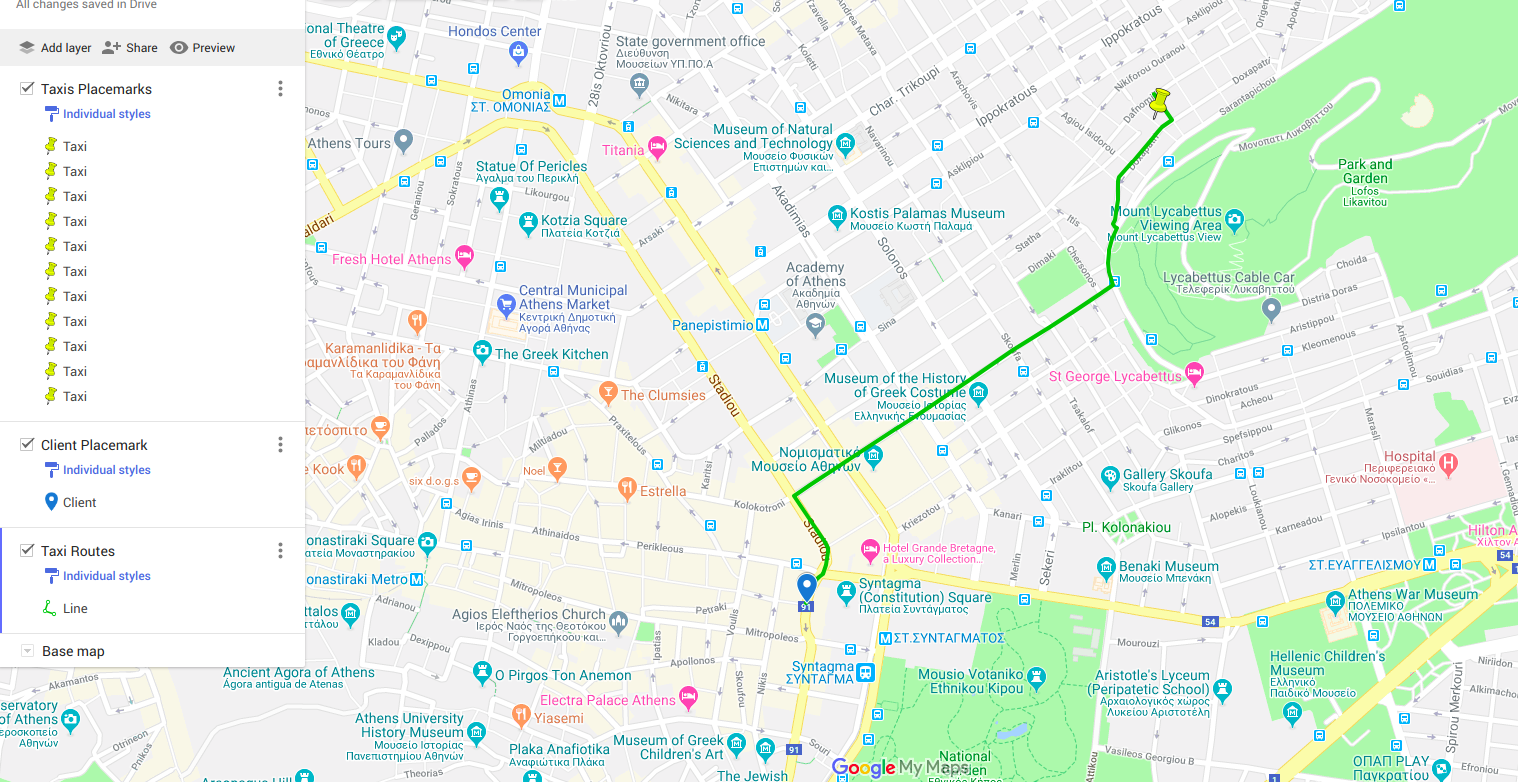
\includegraphics[width=\textwidth]{solution.png}
\end{figure}

\subsection{Εναλλακτικές διαδρομές στα δεδομένα εκφώνησης}
Στα ίδια δεδομένα, αν αλλάξουμε το tolerance παίρνουμε περισσότερες εναλλακτικές διαδρομές που θεωρούνται και αυτές βέλτιστες. Για παράδειγμα, για tolerance = 2m έχουμε τις ακόλουθες διαδρομές που φαίνονται στα ακόλουθα σχήματα (με ή χωρίς ζουμ στις επιμέρους διαδρομές):

\begin{figure}[H]
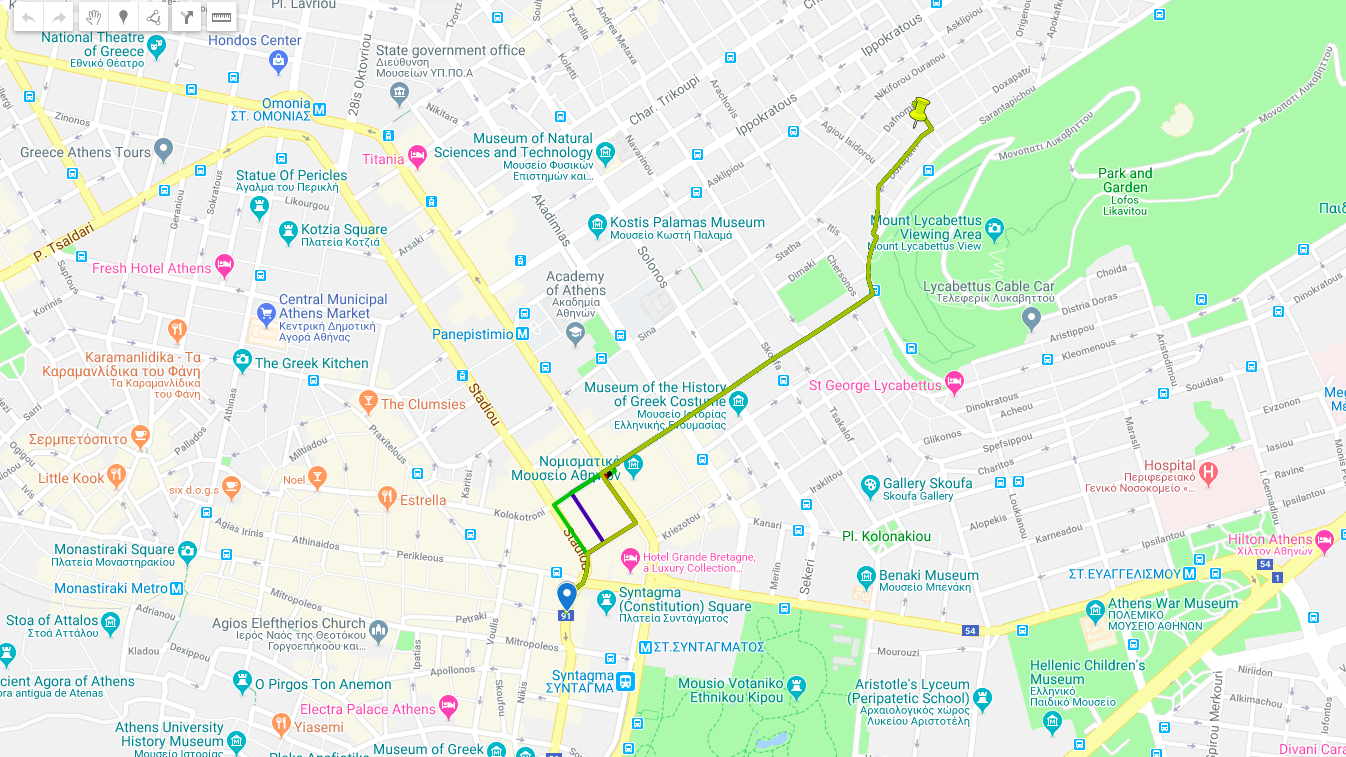
\includegraphics[width=\textwidth]{alt1.png}
\end{figure}

\begin{figure}[H]
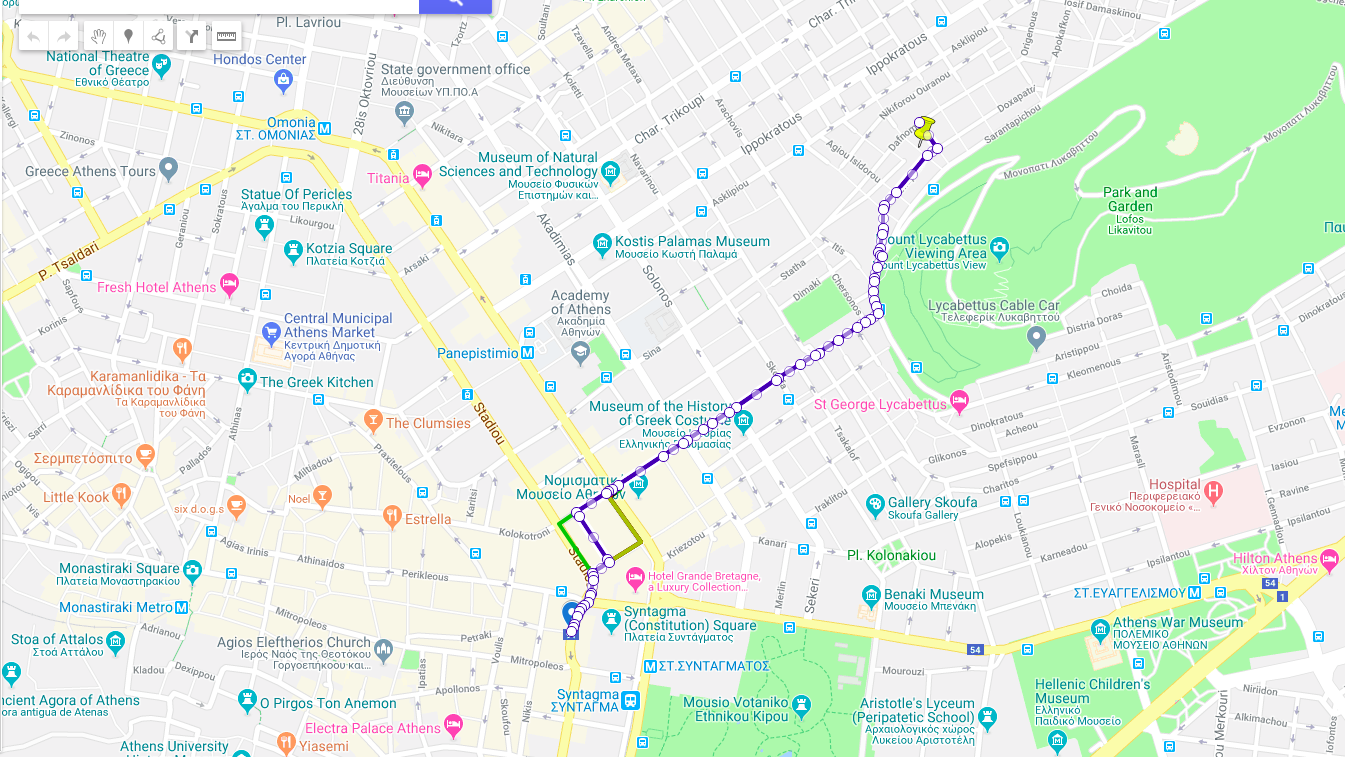
\includegraphics[width=\textwidth]{alt2.png}
\end{figure}


\begin{figure}[H]
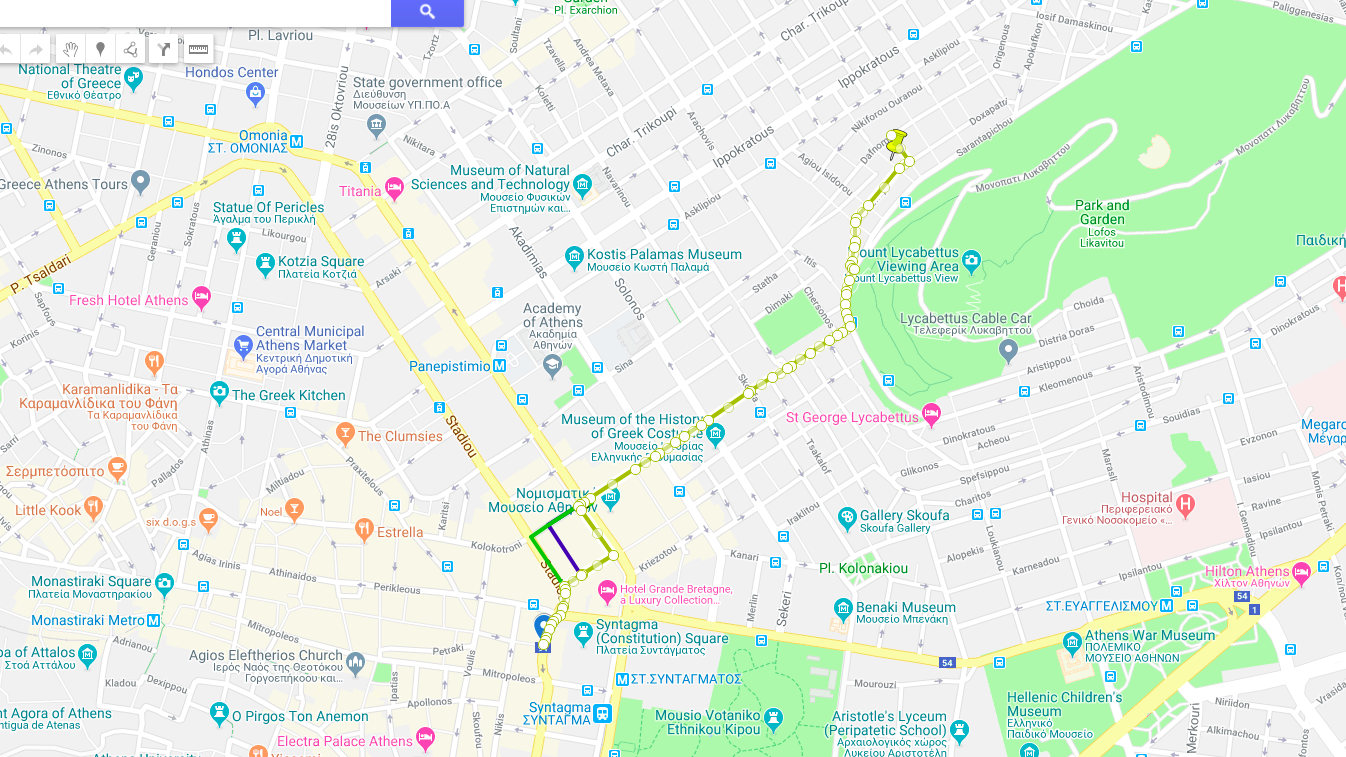
\includegraphics[width=\textwidth]{alt3.png}
\end{figure}


\subsection{Βέλτιστη διαδρομή σε δικά μας δεδομένα}
Για να δούμε ότι ο αλγόριθμος μας δουλέυει σωστά, αλλάζουμε την τοποθεσία του client και τον στέλνουμε αρκετά κοντά σε ένα άλλο ταξί. Για παράδειγμα, ορίζουμε ως client:
$$
23.7831089,38.0278518
$$
Τότε, με tolerance=0 έχουμε την ακόλουθη βέλτιστη διαδρομή:

\begin{figure}[H]
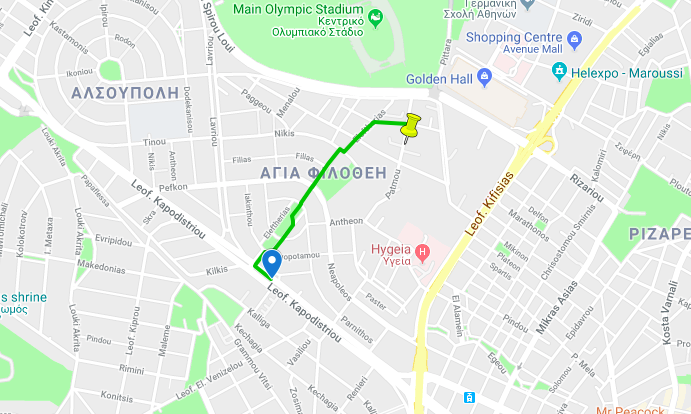
\includegraphics[width=\textwidth]{solution_custom.png}
\end{figure}


\subsection{Εναλλακτικές διαδρομές σε δικά μας δεδομένα}
Τέλος, αλλάζοντας το tolerance μπορούμε να πάρουμε και άλλες βέλτιστες εναλλακτικές διαδρομές:

\begin{figure}[H]
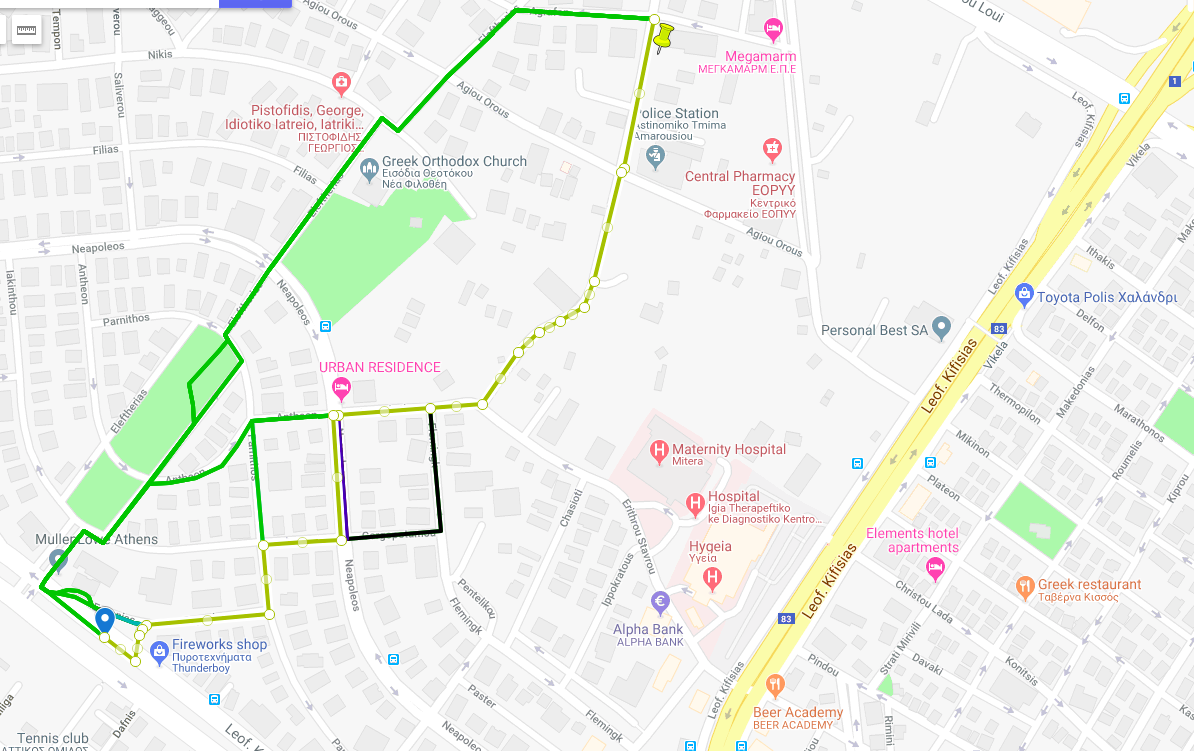
\includegraphics[width=\textwidth]{alt4.png}
\end{figure}

Σημειώνουμε ότι αυτές οι διαδρομές πάρθηκαν με μεγάλο tolerance και συνεπώς υπάρχει απόκλιση 40m από τη βέλτιστη.

\section{Απαντήσεις σε ερωτήσεις εκφώνησης}

Ο αλγόριθμος μας αλλάζοντας το tolerance μπορεί να προτείνει πολύ μεγάλο αριθμό εναλλακτικών διαδρομών. Tolerance της τάξης του 2-5m αντιστοιχεί σε πραγματικά ισοδύναμες διαδρομές, όπως αυτές που προτείνει το Google Maps όταν βάζεις έναν προορισμό και μια αρχή. Μεγαλύτερα tolerance αντιστοιχούν σε διαφορετικούς τρόπους να φτάσεις στον προορισμό αλλά όχι πάντα optimal. Βέβαια πάντα εδώ υπάρχει το ζήτημα του ορισμού του optimal όταν χειριζόμαστε floats αριθμούς ή/και πολύ μεγάλες αποστάσεις. \bigbreak 

Σε κάθε περίπτωση ο αλγόριθμος μας υπάρχει περίπτωση να μη βρίσκει κάποια εναλλακτική βέλτιστη διαδρομή καθώς μπορεί να τερματίσει πριν τη βρεί. Αυτό είναι το tradeoff του να χρησιμοποιείς heuristics; κάνεις πολύ γρήγορα τη διάσχιση ενός τεράστιου χώρου αλλά δεν τον διασχίζεις ολόκληρο.


\section{Βιβλιογραφία}
\noindent [1] Hart, P. E.; Nilsson, N. J.; Raphael, B. (1972). "Correction to "A Formal Basis for the Heuristic Determination of Minimum Cost Paths"". \par 
\noindent[2] Nilsson, N. J. (1980). Principles of Artificial Intelligence. Palo Alto, California: Tioga Publishing Company \par 
\noindent[3] Pohl, Ira (1970). "First results on the effect of error in heuristic search". Machine Intelligence \par 
\noindent[4] Köll, Andreas; Hermann Kaindl (August 1992). "A new approach to dynamic weighting". Proceedings of the Tenth European Conference on Artificial Intelligence \par 
\noindent [5] Stanford online courses \par 
\noindent [6] Oracle Java Docs \par 



\end{document}

